\begin{figure}[h!]
    \centering
    \begin{subfigure}
        \centering
        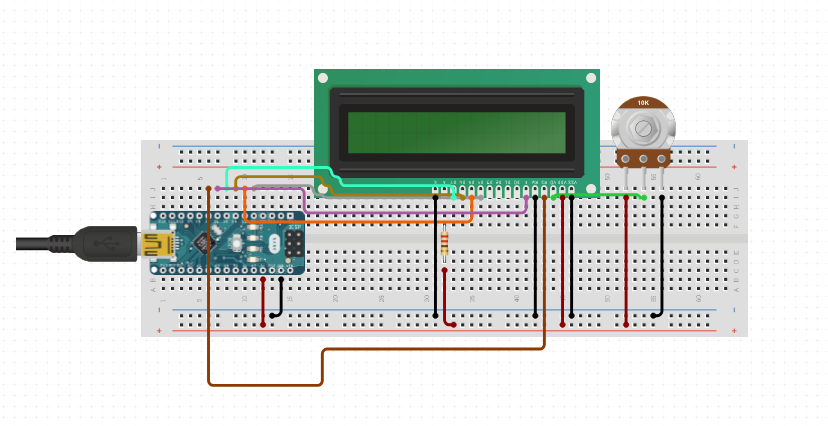
\includegraphics[width=\textwidth,keepaspectratio]{figures/circuit_rx.png}
        \caption{Circuit of Tx}
        \label{fig:Figure 5}
    \end{subfigure}
    \hfill
    \begin{subfigure}
        \centering
        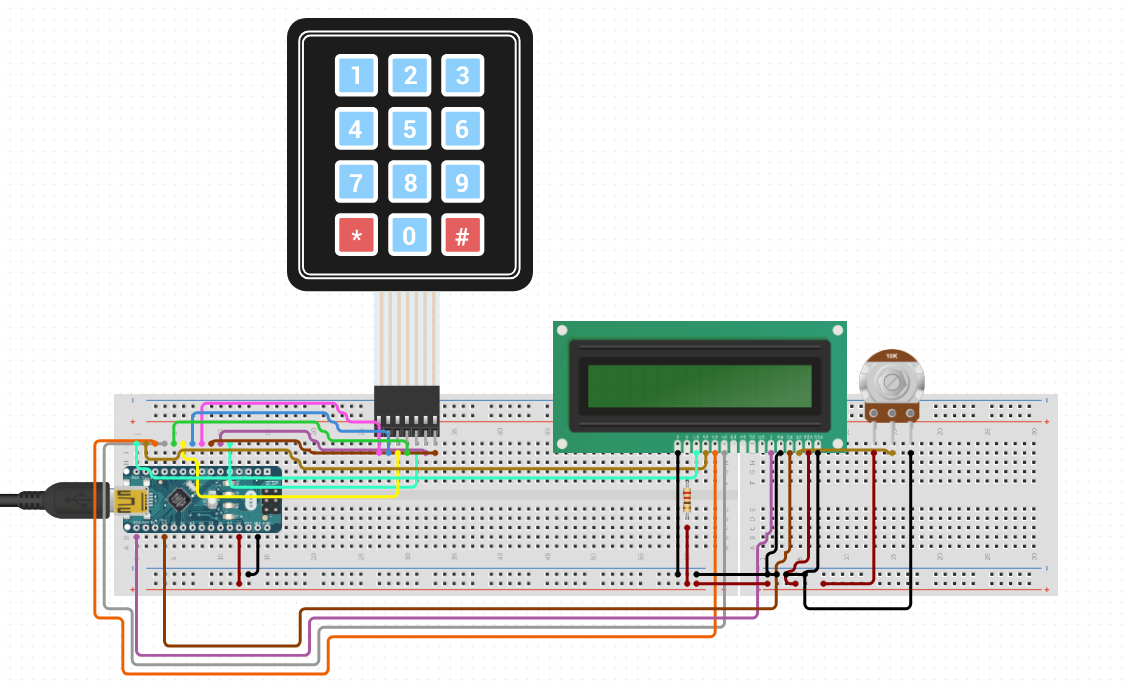
\includegraphics[width=\textwidth,keepaspectratio]{figures/circuit_tx.png}
        \caption{circuit of transmitter}
        \label{fig:Figure 6}
    \end{subfigure}
    % \caption{Overall caption for both images.}
    \label{fig:side_by_side_images}
\end{figure}